


To get started with talking about reinforcement learning,
we need to define the most basic concept, the
\emph{environment} for the decision taking \emph{agent}.
This environment is formalized so called \emph{decision process}.
In order to define this we need the concept of a \emph{probability kernel}

\begin{defn}[Probability kernel]
  Let $(\Cal{X}, \Sigma_\Cal{X}), (Y, \Sigma_\Cal{Y})$ be measurable spaces.
  A function
  \[ \kappa(\cdot \mid \cdot) : \Sigma_\Cal{Y} \times \Cal{X} \to [0,1] \]
  is a $(\Cal{X}, \Sigma_\Cal{X})$-\defemph{probability kernel}
  on $(\Cal{Y}, \Sigma_\Cal{Y})$ provided
  \begin{enumerate}
    \item $B \mapsto \kappa(B \mid x) \in \Cal{P}(\Sigma_\Cal{Y})$
      that is $\kappa(\cdot \mid x)$ is a probability measure
      for any $x \in \Cal{X}$.
    \item
      $x \mapsto \kappa(B \mid x) \in \Cal{M}(\Sigma_\Cal{X}, \Sigma_\Cal{Y})$
      that is $\kappa(B \mid \cdot)$ is ($\Sigma_\Cal{X}$-$\Sigma_\Cal{Y}$)
      measurable for any $B \in \Sigma_\Cal{Y}$.
  \end{enumerate}
  We then write $\kappa : \Cal{X} \leadsto \Cal{Y}$.
  \label{defn:probKer}
\end{defn}

The following example shows how probability kernels are easily constructed.
\begin{example}
  If $f : \cl{X} \times \cl{Y} \to \R$ is positive a measurable function with
  the property that
  \[ \forall x \in \cl{X} : \int f(x, y) \difd \mu(y) = 1 \]
  then $\kappa(B \mid x) = \int_B f(x, y) \difd \mu(y)$ defines a
  $\cl{X}$-probability kernel on $\cl{Y}$.
  %todo proof
\end{example}

A handy property of kernels is
\begin{prop}
  Let $\kappa : \Cal{X} \to \Cal{Y}$ be a probability kernel
  and $f : \cl{X} \times \cl{Y} \to \ol{\ul{\R}}$ be measurable satisfying
  that $f(x, \cdot)$ is $\kappa(\cdot \mid x)$-integrable for every $x \in \cl{X}$.
  Then $x \mapsto \int f \difd \kappa(\cdot \mid x)$ is measurable
  into $(\ol{\ul{\R}}, \ol{\ul{\bb{B}}})$.
  \label{prop:intKerMeas}
\end{prop}
\begin{proof}[Proof of \cref{prop:intKerMeas}]
  Simple functions are measurable since $\kappa$ is a kernel.
  Now extend by sums and limits.
\end{proof}
Here we denote $\Rext = \R \cup \{\pm \infty\}$ and $\ol{\R} = \R \cup \{\infty\}$,
$\ul{\R} = \R \cup \{-\infty\}$.
These are endowed with the natural order topology
(\cref{defn:orderTop}) and the Borel $\sigma$-algebra
(\cref{defn:BorelAlg}) obtained from this.

We can now state the definition of a decision process

\begin{defn}[History dependent decision process]
  A (countable)
  \defemph{history dependent decision process} (HDP) is determined by
  \begin{enumerate}
    \item $(\Cal{S}_n, \Sigma_{\Cal{S}_n})_{n \in \N}$ a 
      measurable space of \defemph{states} for each timestep.
    \item $(\Cal{A}_n, \Sigma_{\Cal{A}_n})_{n \in \N}$ a 
      measurable space of \defemph{actions} for each timestep.

      for each $n \in \N \cup \{\infty\}$
      define the \defemph{history} spaces
      \[ \Cal{H}_1 = \Cal{S}_1, \quad
	\Cal{H}_2 = \Cal{S}_1 \times \Cal{A}_1\times \Cal{S}_2,
	\quad \Cal{H}_3 = \Cal{S}_1 \times \Cal{A}_1 \times \Cal{S}_2 \times
      \R \times \Cal{A}_2 \times \Cal{S}_3 \]
      \[ \Cal{H}_n = \Cal{S}_1 \times \Cal{A}_1
	\times \Cal{S}_2 \times \R \times \Cal{A}_2
      \times \Cal{S}_3 \times \R \times \dots \times \Cal{S}_n \]
      \[
	\Cal{H}_\infty = \Cal{S}_1 \times \Cal{A}_1 \times \Cal{S}_2 \times
	\R \times \dots
      \]
    \item $(P_n)_{n \in \N}$ a sequence of
      $\Cal{H}_n \times \Cal{A}_n \leadsto \Cal{S}_{n+1}$ probability kernels
      called the \defemph{transition} kernels.
    \item $(R_n)_{n \in \N}$ a sequence of
      $\Cal{H}_{n+1} \leadsto \R$ probability kernels
      called the \defemph{reward} kernels.
    \item $A_n(h_n) \subseteq \cl{A}_n$ a set of admissable actions
      for each $h_n \in \cl{H}_n$ and $n \in \N$.
  \end{enumerate}
  \label{sett:HDP}
\end{defn}

%todo example
With a HDP and an a way of choosing actions for each new state
we can obtain sequence of states, actions and rewards, that is
a history, by sampling from the kernels.
%todo example
To make precise what it means to choose actions we introduce the notion
of a \emph{policy}.

\begin{defn}[Policy]
  A (randomized) \defemph{policy} $\pi = (\pi_n)_{n \in \N}$ for a
  HDP is a sequence of probability kernels 
  $\pi_n : \Cal{H}_n \leadsto \Cal{A}_n$,
  such that $\pi_n(A(h_i) \mid h_i) = 1$ for alle $h_i \in \cl{H}_i$,
  i.e. the policy chooses only admissable actions (with probability 1).
  The set of all policies we denote $R\Pi$.
\end{defn}

With a HDP, a starting state $S_1$ and a policy $\pi$ intuitively we
should be able to obtain a history by sampling
\begin{itemize}
  \item an action $A_1 \in A(H_1)$ from $\pi_1(\cdot \mid H_1)$
    (where $H_1 = S_1$),
  \item a state $S_2 \in P(H_2)$ from $P(\cdot \mid H_1, A_1)$,
  \item a reward $R_1 \in \R$ from  $R_1(\cdot \mid H_2)$,
  \item an action $A_2 \in A(H_2)$ from $\pi_2(\cdot \mid H_2)$
  \item and so on.
\end{itemize}

To make this precise we need some additional measure theory on
probability kernels.

\begin{thm}[Integration of a kernel]
  Let $\mu \in \Cal{P}(\Cal{X})$ and $\kappa : \Cal{X} \leadsto \Cal{Y}$.
  Then there exists a uniquely determined probability measure
  $\lambda \in \Cal{P}(\Sigma_\Cal{X} \otimes \Sigma_\Cal{Y})$
  such that
  \[ \lambda(A \times B) = \int_A \kappa(B, x) \difd \mu(x) \]
  \label{thm:intKer}
  We denote this measure $\lambda = \kappa \mu$.
\end{thm}
\begin{proof}
  For $G \in \Sigma_\cl{X} \otimes \Sigma_\cl{Y}$ and $x \in \cl{X}$ define
  $G^x \defeq \{ y \in \cl{Y} \mid (x, y) \in G \} $.
  It is easy to check that the map $x \mapsto \kappa(G^x \mid x)$ is
  measurable, using a Dynkin class argument.
  Thus we can define
  \[ \lambda(G) = \int \kappa(G^x \mid x) \difd \mu(x) \]
  Using this definition we see that
  $\lambda(\cl{X} \times \cl{Y}) = 1$ and by monotone convergence
  for disjoint $G_1, G_2, \dots$
  \[ \lambda \left( \bigcup_{i \in \N} G_i \right)
    = \int \sum_{i=1}^\infty P_x(G^x_n) \difd \mu(x)
  = \sum_{i=1}^\infty \lambda (G_i) \]
  Uniqueness follows because the property
  \[ \lambda(A \times B) = \int_A \kappa(B, x) \difd \mu(x) \]
  should hold on the all product sets, which form an
  intersection-stable generating collection for
  $\Sigma_\cl{X} \otimes \Sigma_\cl{Y}$.
\end{proof}

\begin{rem}
  In light of \cref{thm:intKer} we can view a probability kernel as a mapping
  $\kappa : \cl{P}(X) \leadsto \cl{P}(\cl{X} \times \cl{Y})$
  defined by $\mu \mapsto \kappa \mu$.
  \label{rem:measureMap}
\end{rem}

\begin{defn}[Composition of kernels]
  Let $\kappa : \cl{X} \leadsto \cl{Y}$ and
  $\phi : \cl{X} \times \cl{Y} \leadsto \cl{Z}$ be probability kernels.
  We define the composition $\phi \kappa : \cl{X} \leadsto \cl{Z}$ by
  \[ \phi \kappa(C \mid x) = \int \phi(C \mid x, y) \difd \kappa(y \mid x) \]
  \label{defn:compKer}.
\end{defn}

\begin{rem}
  Following \cref{rem:measureMap} $\phi \kappa$ can be viewed as a mapping
  a from from $\cl{P}(\cl{X})$ to $\cl{P}(\cl{X}\times\cl{Z})$. This is
  somewhat unsatisfactory. We are missing the intermediary space $\cl{Y}$.
  However writing $\phi(\kappa \mu)$ we obtain a measure on
  $\cl{P}(\cl{X} \times \cl{Y} \times \cl{Z})$ as wanted.
  We will therefore use a slight abuse of notation and interpret compositions
  of kernels as including all intermediary spaces,
  when viewed as maps of measures, that is we will write
  $\phi\kappa\mu \in \cl{P}(\cl{X} \times \cl{Y} \times \cl{Z})$.
  It is a trivial exercise to verify that composition when viewed this way
  is associative. That is if $\psi : \cl{X} \times \cl{Y} \times \cl{Z}
  \leadsto \cl{W}$
  is another probability kernel, then
  $((\psi \phi) \kappa) \mu = (\psi (\phi \kappa)) \mu$.
  \label{rem:abuseKernel}
\end{rem}

\begin{rem}
  When one has $\varphi:\cl{Y} \to \cl{Z}$ we can also use \cref{defn:compKer}
  since $\varphi$ can be viewed as a $\cl{X}\times\cl{Y}$-kernel which does
  not depend on its input from $\cl{X}$.
  We write $\varphi \circ \kappa : \cl{X} \leadsto \cl{Z}$.
  This is often also referred to a \emph{composition of kernels}.
  In fact it makes the class of measurable spaces
  into a category \mcite{L62},
  with identity $\id_{\Cal{X}}(\cdot \mid x) = \delta_x$.
\end{rem}

\begin{rem}
  Let $(\Cal{X}_n, \Sigma_{\Cal{X}_n})_{n \in \N}$ be a sequence
  of measurable spaces. For each $n \in \N$ define
  $\Cal{X}^{\ul{n}} \defeq \Cal{X}_1 \times \dots \times \Cal{X}_n$,
  $\Sigma_{\Cal{X}^{\ul{n}}} \defeq \Sigma_{\Cal{X}_1} \otimes
  \dots \otimes \Sigma_{\Cal{X}_n}$
  and let
  $\kappa_n : \Cal{X}^{\ul{n}} \leadsto \Cal{X}_{n+1}$ be a probability kernel.
  Then by \cref{rem:abuseKernel}
  $\kappa^{\ul{n}} \defeq \kappa_n \dots \kappa_1$ defines a map
  from $\cl{P}(\cl{X}_1)$ to $\cl{P}(\Cal{X}^{\ul{n+1}})$.
\end{rem}

\Cref{rem:abuseKernel} allows us to make sense to finite decision processes.
That is for any
$n \in \N$, distribution $\mu \in \cl{P}(\cl{S}_1)$ of $S_1$ 
and policy $(\pi_1, \pi_2, \dots) \in R\Pi$ we can get a distribution
of the $n$th history $H_n \in \cl{H}_n$ by the composition of kernels
\[ P_{n-1} \pi_{n-1} R_{n-2} P_{n-2} \pi_{n-2}
\dots R_2 P_2 \pi_2 R_1 P_1 \pi_1 \mu \in \cl{P}(\cl{H}_n) \]
We would like to extend this to a distribution on $\cl{H}_\infty$.
To do this we will need

\begin{thm}[Ionescu-Tulcea extension theorem]
  For every $\mu \in \Cal{P}(\Cal{X}_1)$ 
  there exists a unique probability measure
  $\rho \in \Cal{P}(\Cal{X}^{\ul{\infty}})$ such that
  \[ \kappa^{\ul{n-1}} \mu (A) = \rho
    \left( A \times \prod_{k=n+1}^\infty \Cal{X}_k \right)
  , \qquad \forall A \in \Sigma_{\Cal{X}^{\ul{n}}}, n \in \N \]
  \label{thm:ionescuTulcea}
\end{thm}
\begin{proof}
  We refer to \mcite{K02} thm. 5.17. %todo do the proof instead
\end{proof}

It is even possible to view the Ionescu-Tulcea construction as a kernel

\begin{prop}[Ionescu-Tulcea kernel]
  Let $\mu_x$ denote the Ionescu-Tulcea measure of a
  sequence of probability kernels
  $\kappa_i : \Cal{X}^{\ul{i}} \to \Cal{X}_{i+1}$
  with starting measure $\delta_x$ on $\Cal{X}_1$ for any $x \in \Cal{X}_1$.
  Then $\kappa(A \mid x) = \mu_x(A)$ defines a probability kernel
  $\kappa : \Cal{X}_1 \to \Cal{X}^{\ul{\infty}}$.
\end{prop}
\begin{proof}
  Since we already know that $\mu_x$ is a probability measure for any
  $x \in \Cal{X}_1$,
  we just have to show that $\kappa(A \mid x) = \mu_x(A)$ is measurable
  as a function of $x$ for all
  $A \in \Sigma_{\Cal{X}^{\ul{\infty}}}
  = \bigotimes_{i=1}^\infty \Sigma_{\Cal{X}_i}$.
  Let $\phi_A = x \mapsto \mu_x(A)$
  for all $A \in \Sigma_\Cal{X^{\ul{\infty}}}$ and define
  \[ \bb{G} = \left\{ A \in \bigotimes_{i=1}^\infty \Sigma_{\Cal{X}_i}
  \Mid \phi_A \in \Cal{M}(\Sigma_{\Cal{X}_1}, \bb{B}_{[0,1]}) \right\} \]
  The cylinder algebra
  \[ \bb{O} = \left\{ A_1 \times \dots \times A_i \times \Cal{X}_{i+1},
  \dots \Mid A_i \in \Sigma_{\Cal{X}_i}, i \in \N \right\} \]
  is a generator for $\Sigma_{\Cal{X}^{\ul{\infty}}}$ stable under 
  finite intersections.
  By contruction $\bb{O} \subseteq \bb{G}$ since
  \[ \phi_{A_1 \times \dots \times A_i \times \Cal{X}_{i+1} \times \dots}
  = \kappa^{\ul{i-1}}(A_1 \times \dots \times A_i \mid \cdot) \]
  and any $\kappa^{\ul{i-1}}$ is a kernel making that function measurable.
  We will show that $\bb{G}$ is a Dynkin class.
  Then by Dynkins $\pi$-$\lambda$ theorem (see \cref{thm:DynkinPiLambda})
  \[ \sigma(\bb{O}) = \Sigma_{\Cal{X}^{\ul{\infty}}}
  \subseteq \bb{G} \]
  implying that $\phi_A$ is measurable
  for all $A \in \Sigma_{\Cal{X}^{\ul{\infty}}}$.
  
  Clearly $\Cal{X}^{\ul{\infty}}, \emptyset \in \bb{G}$ and if
  $A,B \in \bb{G}$ with $A \subseteq B$ then
  $\phi_{B \setminus A} = \phi_B - \phi_A \in \bb{G}$.
  Finally if $(B_n)_{n \in \N}$ is an ($\subseteq$-) increasing sequence
  in $\bb{G}$ then $\phi_{\bigcup_{n=1}^\infty B_n} =
  \lim_{n \to \infty} \phi_{B_n}$ is again measurable as it is a
  limit of measurable functions, showing that $\bb{G}$ is a Dynkin class.
\end{proof}

We will denote the Ionescu-Tulcea kernel $\dots \kappa_2 \kappa_1$ or
$\prod_{i=1}^\infty \kappa_i$ or simply $\kappa^{\ul{\infty}}$.
The next lemma will come in handy when manipulating with integrals over
kernel derived measures.

\begin{lem}
  The Ionescu-Tulcea kernel satisfies
  $\prod_{i=1}^\infty \kappa_i = (\prod_{i=2}^\infty \kappa_i) \kappa_1 $.
  \label{lem:ionescu}
\end{lem}
\begin{proof}
  Let $x \in \Cal{X}_1$.
  Notice that by associativity of the composition of finitely many
  kernels
  $\kappa_n \dots \kappa_1 \mu
  = (\kappa_n \dots \kappa_2) (\kappa_1 \mu)$.
  This implies that
  \[ \left( \prod_{i=1}^\infty \kappa_i \mu \right)
    \left( A \times \prod_{k=n+1}^\infty \Cal{X}_k \right)
    = \left( \left( \prod_{i=2}^\infty \kappa_i \right) \kappa_1 \mu \right)
  \left( A \times \prod_{k=n+1}^\infty \Cal{X}_k \right) \]
  for all $n \in \N$ and $A \in \Sigma_{\Cal{X}^{\ul{n}}}$.
  By the uniqueness in \cref{thm:ionescuTulcea} we are done.
\end{proof}

Let $\mu \in \cl{P}(\cl{S}_1)$ be a measure on the first state space.
By \cref{thm:ionescuTulcea} a HDP and a policy $\pi$ gives rise to
a kernel $\kappa_\pi : \cl{P}(\cl{S}_1) \to \cl{P}(\cl{H}_\infty)$, namely
\begin{equation}
  \kappa_\pi = \dots R_2 P_2 \pi_2 R_1 P_1 \pi_1 \mu
  \label{eq:kappaPi}
\end{equation}
In particular $\kappa_\pi \mu$ can be interpreted as the stochastic process
arising from sampling the first state from $\mu$ and then follow $\pi$
for a countable number of steps.
We will denote expectation with respect to $\kappa_\pi \mu$ by
$\E_{\mu}^\pi$. 
In the case where 
$\kappa_\pi \delta_{s}$ can be interpreted as the stochastic process
arise from starting in state $s$ and following policy $\pi$.
We will abuse notation slightly, writing
$\kappa_\pi \delta_s = \kappa_\pi s$ and $\E_{\delta_s}^\pi = \E_s^\pi$.

\section{Policy evaluation and value functions}
The next step is to evaluate how \emph{good} a policy is.
To this end we introduce \emph{value functions}.
In order for the sum of finitely many rewards
to have a meaningful expected value
we will need one of
the following conditions:

\begin{cond}{$F^-$}[Reward finity from above]
  $\int_{[0,\infty]} x \difd R_i(x \mid h) < \infty$ for all
  $h \in \Cal{H}_{i+1}$ and $i \in \N$
  \label{cond:F-}
\end{cond}
\begin{cond}{$F^+$}[Reward finity from below]
  $\int_{[-\infty,0]} x \difd R_i(x \mid h) > -\infty$ for all
  $h \in \Cal{H}_{i+1}$ and $i \in \N$
  \label{cond:F+}
\end{cond}

Under $(F^+)$ or $(F^-)$ following definition makes sense 
\begin{defn}[Finite horizon value function]
  Let $\ul{R}_i : \Cal{H}_\infty \to \Rext$ be the projection map onto the
  $i$th reward. We define the function $V_{n, \pi} : \cl{S}_1 \to \Rext$ by
  \[ V_{n,\pi}(s_1) = \E_s^\pi \sum_{i=1}^n \ul{R}_i \]
  called the $k$th finite horizon value function.
  When $n=0$ we say $V_{0,\pi} = V_0 \defeq 0$ for any $\pi$.
\end{defn}
The finite horizon value function
measures the expected total reward of starting in state $s$
and then follow the policy $\pi$ for $n$ steps.
This way it measures the \emph{value} of that particular state
given a policy and \emph{horizon} (number of steps).

We would like to extend this to an infinite horizon value function,
i.e. letting $n$ tend to $\infty$. To ensure that the integral is well-defined
we introduce the following conditions
\begin{cond}{P}[Reward non-negativity] $R_i([0,\infty] \mid h) = 1$,
  $\forall h \in \Cal{H}_{i+1}, i \in \N$
  \label{cond:P}
\end{cond}
\begin{cond}{N}[Reward non-positivity] $R_i([-\infty, 0] \mid h) = 1$
  $\forall h \in \Cal{H}_{i+1}, i \in \N$
  \label{cond:N} 
\end{cond}
\begin{cond}{D}[Discounting] There exist a bound $R_{\max} > 0$ and a
  $\gamma \in [0,1)$ called the \defemph{discount} factor such that
  $R_i([-R_{\max} \gamma^i, R_{\max} \gamma^i]) = 1$
  $\forall h \in \Cal{H}_{i+1}, i \in \N$
  \label{cond:D}
\end{cond}
\begin{rem}
  The letters $F^+, F^-$, P, N and D are adopted from \ncite{BS07}. 
\end{rem}
\begin{defn}
  We define the infinite horizon value function by
  \[ V_\pi(s) = \E_s^\pi \lim_{n \to \infty} \sum_{i=1}^n \ul{R}_i \]
\end{defn}
The infinite horizon value function $V_\pi$ measures the expected total
reward after following the policy $\pi$ an infinite number of steps.

\begin{rem}
  Whenever we are working with the finite horizon value function
  we will always assume that either ($F^+$) or ($F^-$) holds without
  stating this explicitly.
  If a result only holds under e.g. ($F^+$) we will of course be explicit
  about this be marking it accordingly with a ($F^+$).

  Similarly whenever we work with the infinite horizon value function we will
  always assume that at least one of (P), (N) or (D) holds.
  We will mark propositions and theorems
  by e.g. (\cref{cond:D}) (\cref{cond:P}) when
  the result only holds for if discounting \emph{or} reward non-negativity
  is assumed.
  Note that obviously (P) implies $F^+$ and (N) implies $F^-$.
\end{rem}

We mention some immediate properties of the finite and infinite horizon
value functions
\begin{prop}
  \leavevmode
  \begin{enumerate}
    \item $V_{n,\pi}, V_\pi$ are measurable
      into $(\ul{\ol{\R}}, \ul{\ol{\bb{B}}})$
      and under (D) they are integrable with respect to $\kappa_\pi(\cdot \mid s)$
      for any $\pi \in R\Pi$.
    \item $\lim_{n\to\infty} V_{n, \pi} = V_\pi $
      for all $\pi \in R\Pi$.
    \item Under (D) for any $\pi \in R\Pi$
      \[\abs{V_{n,\pi}}, \abs{V_\pi} \leq R_{\max} (1 - \gamma) < \infty\]
  \end{enumerate}
  \label{prop:VpiMeas}
\end{prop}
\begin{proof}  
  \leavevmode
  \begin{enumerate}
    \item Use \cref{prop:intKerMeas}.
    \item By monotone or dominated convergence.
    \item For any $\pi \in R\Pi$
      \[ \abs{V_\pi(s)} \leq \E_s^\pi \sum_{i \in \N} \abs{\ul{R}_i}
	\leq \sum_{i \in \N} \gamma^{i-1} R_{\max}
      = R_{\max} / (1-\gamma) \]
      This also covers $V_{n, \pi}$.
  \end{enumerate}
\end{proof}

\begin{rem}
  As this bound will occur again and again we denote it
  \begin{equation}
    V_{\max} \defeq R_{\max}(1-\gamma)
    \label{eq:VmaxDef}
  \end{equation}
\end{rem}

\subsection{The optimal value function}

\begin{defn}[Optimal value functions] 
  \begin{align*}
    V_n^*(s) \defeq & \; \sup_{\pi \in R\Pi} V_{n,\pi}(s) &
    V^*(s) \defeq & \; \sup_{\pi \in R\Pi} V_\pi(s)
  \end{align*}
  This is called the \defemph{optimal value function} (and the $n$th
  optimal value function).
  A policy $\pi^* \in R\Pi$ for which $V_{\pi^*} = V^*$ is called an
  \defemph{optimal policy}.
  If $V_{n, \pi^*} = V^*_n$ it is called $n$-optimal.
  \label{defn:optimalValue}
\end{defn}

\begin{prop} Under (D) we have
  $\abs{V^*_k},\; \abs{V^*} \leq V_{\max}$.
\end{prop}
\begin{proof}
  All terms in the suprema are within this bound.
\end{proof}

\begin{rem}
It is known that the optimal value function
might not be Borel measurable (see ex. 2 p. 233 \ncite{BS07}).
Perhaps this is not suprising since we are taking a supremum over
sets of policies which might have cardinality of at least the continuum.
\end{rem}

At this point some relevant questions can be asked.
\begin{enumerate}
  \item To which extend does an optimal policy $\pi^*$ exist?
  \item Does $V_n^*$ converge to $V^*$?
  \item When can optimal policies be chosen to be Markov, deterministic, etc.?
  \item Can an algorithm be designed to efficiently find $V^*$ and
    $\pi^*$?
\end{enumerate}

In a quite general setting, questions 1 and 2
is investigated in \mcite{S75}.
Here some additional structure on our process is imposed.
\begin{defn}[Standard Borel measurable space]
  A measurable space $(\cl{X}, \Sigma_\cl{X})$ is called
  \defemph{standard Borel} if $\cl{X}$ is Polish space, that is a
  seperable completely metrizable space, and $\Sigma_\cl{X}$ is
  the Borel $\sigma$-algebra of $\cl{X}$, that is the $\sigma$-algebra
  generated by all open sets.
  \label{defn:standardBorelp}
\end{defn}
\begin{sett}[Schäl]
  \leavevmode
  \begin{enumerate}
    \item $V_\pi < \infty$ for all policies $\pi \in R\Pi$.
    \item $(\Cal{S}_n, \Sigma_{\Cal{S}_n})$ are all standard Borel.
    \item $(\Cal{A}_n, \Sigma_{\Cal{A}_n})$ are all standard Borel.
    \item The set of admissible actions
      $A_n(h_n)$ is compact for any $h_n \in \cl{H}_n, \; n \in \N$.
    \item The kernels $(P_n, R_n)_{n \in \N}$ are independent of 
      rewards in the process.
    \item 
      $ \forall s \in \Cal{S}_1 :
	Z_n = \sup_{N \geq n} \sup_{\pi \in R\Pi} \sum_{t=n+1}^N
      \E_s^\pi \ul{R}_n \to 0, \quad n \to \infty $
  \end{enumerate}
  \label{sett:Schal}
\end{sett}

In this setting Schäl introduced two sets of criteria for the existence
of an optimal policy:

\begin{cond}{S}
  \leavevmode
  \begin{enumerate}
    \item The function \[
	(a_1, a_2, \dots, a_n) \mapsto
	P_n(\cdot \mid s_1, a_1, s_2, a_2, \dots, s_n, a_n)
      \]
      is set-wise continuous (hence the name \defemph{S})
      for all $s_1, \dots, s_n \in \Cal{S}^{\ul{n}}$.
    \item $r_n$ is upper semi-continuous.
  \end{enumerate}
  \label{cond:S}
\end{cond}

\begin{cond}{W}
  \leavevmode
  \begin{enumerate}
    \item The function
      \[(h_n, a_n) \mapsto P_n(\cdot \mid h_n, a_n)\]
	is weakly continuous (hence the name \defemph{W}).
    \item $r_n$ is continuous.
  \end{enumerate}
  \label{cond:W}
\end{cond}

\begin{thm}[Schäl]
  Under \cref{sett:Schal} when either (\cref{cond:S}) or (\cref{cond:W}) hold
  then
  \begin{enumerate}
    \item There exist an optimal policy $\pi^* \in R\Pi$.
    \item $V^*_n \to V^*$ as $n \to \infty$.
  \end{enumerate}
  \label{thm:SchalExi}
\end{thm}
\begin{proof}
  We refer to \ncite{S75}. %todo: or do we?
\end{proof}

\begin{cor}
  Under \cref{sett:Schal} when either (\cref{cond:S}) or (\cref{cond:W}) hold then
  $V^*$ is (Borel) measurable.
\end{cor}
\begin{proof}
  Since by \cref{thm:SchalExi} there exists an optimal policy $\pi^*$ we have
  $V^* = V_{\pi^*}$ which is measurable due to \cref{prop:VpiMeas}.
\end{proof}

Schäls theorem tells us that optimal policies exist in a wide class
of decision processes. In many cases we are looking at processes
in which the next state in independent of the history,
that is \emph{Markov}.
In such cases it makes sense to ask if optimal policies can be chosen
to also be Markov.
Such questions will be addressed in the next section.

\section{Markov decision processes}

\begin{defn}[Markov decision process]
  A \defemph{Markov decision process} (MDP) consists of
  \begin{enumerate}
    \item $(\Cal{S}, \Sigma_{\Cal{S}})$ a 
      measurable space of states.
    \item $(\Cal{A}, \Sigma_{\Cal{A}})$ a 
      measurable space of actions.
    \item $P : \Cal{S} \times \Cal{A} \leadsto \Cal{S}$
      a transition kernel.
    \item $R : \Cal{S} \times \Cal{A} \leadsto \ol{\ul{\R}}$
      a reward kernel.
    \item An optional disount factor $\gamma \in [0,1]$
      (when not discounting put $\gamma = 1$).
    \item $A(s) \subseteq \cl{A}$ a set of admissable actions
      for each $s \in \cl{S}$.
  \end{enumerate}
  \label{sett:MDP}
\end{defn}
This is a special case of the
history dependent decision process (\cref{sett:HDP}) with
\begin{itemize}
  \item 
    $\Cal{S}_1 = \Cal{S}_2 = \dots = \Cal{S},
    \quad \Cal{A}_1 = \Cal{A}_2 = \dots = \Cal{A}$.
  \item $P_n$ depends only on $s_n$ and $a_n$ and does not
    differ with $n$, i.e. 
    $P_n(\cdot \mid s_1, \dots, s_n, a_n) = P(\cdot \mid s_n, a_n)$
    for all $n \in \N$.
  \item $R_n$ depends only on $s_n$ and $a_n$ and does not differ
    with $n$ except for a potential discount.
    I.e. $R = R_n/\gamma^{n-1}$ for all $n \in \N$
\end{itemize}
We will write $P$ instead of $P_n$ understanding
kernel compositions as if using $P_n$.
\begin{rem}
 Expectations over any reward $R_i$ occuring in an MDP
 can be computed from a function $r: \cl{S} \times \cl{A} \to \Rext$,
 defined by $r(s, a) = \int r' \difd R(r' \mid s, a)$.
 To see this note that
 \begin{align*}
   \E_\mu^\pi \ul{R}_i &= \int \ul{R}_i \difd \kappa_\pi \mu
   \\ &= \int r_i \difd R_i P \pi_i \dots R_1 P \pi_1 \mu
   (s_1, a_1, \dots, s_{i+1}, r_i)
   \\ &= \int \gamma^{i-1} r(s_i, a_i) \difd \pi_i \dots R_1 P \pi_1 \mu
   (s_1, a_1, \dots, s_i, a_i)
   \\ &= \E_\mu^\pi \gamma^{i-1} r(\ul{S}_i, \ul{A}_i)
 \end{align*}
 where $\ul{S}_i, \ul{A}_i$ are projection onto the $i$th state and action.
\end{rem}
\begin{rem}
  One could ask if it is possible to embed a HDP into an MDP
  by setting
  $\Cal{S} \defeq \bigcup_{i\in\N} \Cal{S}_i$ and
  $\Cal{A} \defeq \bigcup_{i\in\N} \Cal{A}_i$ or similar.
  One attempt at this can be found in \ncite{BS07} chapter 10,
  but this will not be covered here. %consider covering it
  Note however that whatever properties, such as those in \cref{sett:Schal},
  one assumes regarding the spaces $\cl{S}_1, \cl{A}_1, \dots$, one must 
  reconsider if each such property hold in the new constructed MDP.
\end{rem}
Intuitively when the environment is a Markov decision process
it should not be necessary that policies depend on the history.
To talk about this topic we introduce

\begin{defn}[Policy classes]
  A policy $\pi = (\tau_1, \tau_2, \dots) \in R\Pi$
  is called \defemph{Markov} if it
  only depends on the last state is the history.
  That is there exist $\tau_1, \tau_2, \dots : \cl{S} \leadsto \cl{A}$
  such that $\tau_i(\cdot \mid s_1, \dots s_i) = \tau_i(\cdot \mid s_i)$.
  We denote the set of (random) Markov policies by $M\Pi$.
  If $\tau_1 = \tau_2 = \dots$ the Markov policy is called
  \defemph{stationary}
  and the set of them denote by $S\Pi$.
  Furthermore $\pi$ is called \defemph{deterministic} if all $\tau_i$
  are degenerate, i.e. for all $i$ we have
  $\tau_i(\{a_i\} \mid h_i) = 1$ for some $a_i \in \Cal{A}_{i}$.
  We denote the deterministic version of the policy classes
  by the letter $D$.
\end{defn}
\begin{rem} 
  We have the following inclusions of policy classes
  \[ \begin{matrix}
      S\Pi &\subseteq M\Pi &\subseteq R\Pi
      \\ \rleft{\subseteq} & \rleft{\subseteq} & \rleft{\subseteq} 
      \\ DS\Pi &\subseteq DM\Pi &\subseteq D\Pi
  \end{matrix} \] 
  Note that stationary policies might not exist
  in HDPs, but always exist for MDPs.
  A policy $(\tau_1, \tau_2, \dots) \in R\Pi$ is deterministic
  if and only if there exist measurable
  functions $\varphi_n : \cl{H}_n \to \cl{A}$ such that
  $\tau_n(\cdot \mid h_n) = \delta_{\varphi_n(h_n)}$. Therefore we shall sometimes
  write $\tau_n(h_n) = \varphi_n(h_n)$, viewing $\tau_n$ as a function.
  For convenience
  will view stationary policies $\tau \in S\Pi$ interchangeably as kernels
  $\tau : \cl{S} \leadsto \cl{A}$ and as the policy
  $(\tau, \tau, \dots)$.
\end{rem}

We will prove that in MDPs under mild assumptions the optimal policy
can be chosen to be deterministic, Markov, and even stationary.
Before we do this we define some important tools for studying MDPs.

\begin{defn}[The $T$-operators]
  For a stationary policy $\tau \in S\Pi$ and measurable $V:\Cal{S} \to \Rext$
  we define the operators 
  \[ T_\tau V \defeq s \mapsto \int r(s, a)
  + \gamma V(s') \difd (P \tau)(a, s'\mid s) \]
  \[ T V \defeq s \mapsto \sup_{a \in A(s)} T_a V(s) \]
  where $T_a = T_{\delta_a}$ for $a \in A(s)$.
\end{defn}
\begin{rem}
  For the integral to make sense we assume under (D) that $V$ is bounded,
  under (P) that $V\geq 0$ and under (N) that $V \leq 0$.
\end{rem}

The $T$ operator is sometimes called the \emph{Bellman-operator}. %todo check this
It is harder to work with than $T_\tau$ because it envolves a supremum.
Therefore we will first take a closer look at properties of $T_\tau$.

\begin{prop}[Properties of the $T_\tau$-operator]
  Let $\pi = (\tau_1, \tau_2, \dots) \in M\Pi$ be a Markov policy,
  and $\tau \in S\Pi$ be a stationary policy.
  \begin{enumerate}
    \item $T_\tau$ is measurable and commutes with limits.
    \item $V_{k, \pi} = T_{\tau_1} V_{k-1, (\tau_2, \dots)}
      = T_{\tau_1} \dots T_{\tau_k} V_0$.
    \item $V_\pi = \lim_{k \to \infty} T_{\tau_1} \dots T_{\tau_k} V_0$
    \item For the stationary policy $\tau$ we have $T_\tau V_\tau = V_\tau$.
    \item (D) $T$ and $T_\tau$ are $\gamma$-contractive
      on $\Cal{L}_\infty(\Cal{S})$.
    \item (D) $V_\tau$ is the unique bounded fixed point of $T_\tau$
      in $\Cal{L}_\infty(\Cal{S})$
  \end{enumerate} 
  \label{prop:propTpiV}
\end{prop}

\begin{rem}
  Here $\cl{L}_\infty(\cl{S})$ denotes the set of essentially bounded
  measurable functions on $\cl{S}$. Since we interested in integration
  with respect to the variety of measures arising as the composition
  $P \circ \tau$ we must assume essential boundedness with respect to
  all such measures. Note that the set of every-bounded measurable functions
  is a subset of $\cl{L}_\infty(\cl{S})$ defined in this way, so it is
  non-empty.
\end{rem}

\begin{proof}[Proof of \cref{prop:propTpiV}]
  \leavevmode
  \begin{enumerate}
    \item Measurability is by \cref{prop:intKerMeas} the rest follows by
      monotone or dominated convergence.
      \label{commLimits}
    \item We have
      \begin{align*}
	&T_{\pi_1} V_{k,(\pi_2, \dots)}(s_1)
	\\ &= \int r(s_1, a_1) + \gamma
	\int \sum_{i=2}^{k+1} \gamma^{i-2} r(s_i, a_i)
	\difd \kappa_{(\pi_2, \dots)} (a_2, s_3, a_3, \dots \mid s_2)
	\difd P \pi_1(a_1, s_2 \mid s_1)
	\\ &= \int \sum_{i=1}^{k+1} \gamma^{i-1} r(s_i, a_i)
	\difd \dots P \pi_2 P \pi_1 (a_1, s_2, \dots \mid s_1)
	\\ &= \int \sum_{i=1}^{k+1} \gamma^{i-1} r(s_i, a_i)
	\difd \kappa_\pi (a_1, s_2, \dots \mid s_1)
	\\ &= V_{k+1, \pi}(s_1)
      \end{align*}
      Now use this inductively.
    \item This is by 2. and a monotone or dominated convergence.
    \item By 3. $T_\pi V_\pi = T_\pi \lim_{k \to\infty} T_{\pi}^k V_0
      = \lim_{k \to\infty} T_\pi^{k+1} V_0 = V_\pi$.
    \item Let $V, V' \in \Cal{L}_\infty(\Cal{S})$
      and let $K = \norm{V - V'}_\infty$.
      Then since the rewards are bounded
      \[ \abs{T^\pi V - T^\pi V'}
	= \gamma \abs{\int V(s') - V'(s') \difd P\pi(s' \mid s)}
      \leq \gamma K \]
      For $T$ use the same argument and the fact that
      $\abs{\sup_x f(x) - \sup_{y} g(y)} \leq
      \abs{\sup_x f(x) - g(x)}$ for any $f,g : X \to \ul{\R}$.
    \item By 4., 5. and Banach fixed point theorem.
  \end{enumerate}
\end{proof}

\subsection{Greedy policies}

\begin{defn}
  Let $\tau : \cl{S} \leadsto \cl{A} \in S\Pi$ be a stationary policy and
  let $V : \cl{S} \to \Rext$ be a measurable value-function.
  We define
  \[ G_V(s) = \argmax_{a \in A(s)} T_a V(s) \subseteq A(s) \]
  as the set of \defemph{greedy} actions w.r.t. $V$.
  If for which there exists a measurable $G_V^\tau(s) \subseteq G_V(s)$
  such that
  \[ \tau(G_V^\tau(s) \mid s) = 1 \]
  for every $s \in \cl{S}$, then $\tau$ is called greedy w.r.t. $V$.
  We will often denote a $V$-greedy policy by $\tau_V$.
\end{defn}

In order to talk about existence of greedy policies we need some additional
structure on our MDP.

\begin{defn}[Borel $\sigma$-algebra]
  For a topological space the \defemph{Borel} $\sigma$-algebra is the smallest
  $\sigma$-algebra containing all open sets.
\end{defn}

\begin{defn}[Weak topology]
  Let $\cl{X}$ be a metrizable space equipped with the Borel $\sigma$-algebra.
  Consider the family of subsets of $\cl{P}(\cl{X})$
  \[ \cl{V} \defeq \left\{ V_\ve(p, f) \Mid \ve > 0, p \in \cl{P}(\cl{X}),
    f \in C(\cl{X}) \right\}, \; \mathrm{where} \;
    V_\ve(p, f) \defeq \left\{ q \in \cl{P}(\cl{X}) \Mid
  \abs{\int f \difd q - \int f \difd p} < \ve \right\} \]
  and where $C(\cl{X})$ denote the set of continuous functions $\cl{X} \to \R$.
  The \defemph{weak} topology on $\cl{P}(\cl{X})$ is the coarsest topology
  containing $\cl{V}$.
\end{defn}

Recall (\cref{defn:standardBorelp}) that a measurable space is
standard Borel if it is Polish and equipped with the Borel $\sigma$-algebra.

\begin{prop}
  Let $\cl{X}$ be a standard Borel measurable space.
  Consider the space $\cl{P}(\cl{X})$ of probabilty measures on $\cl{X}$
  equipped with the weak topology.
  Then $\cl{P}(\cl{X})$ is standard Borel.
  If furthermore $\cl{X}$ is compact then $\cl{P}(\cl{X})$ is also compact.
\end{prop}
%todo proof?
\begin{proof}
  We refer to \ncite{BS07} cor.7.25.1 and prop.7.22.
\end{proof}

\begin{defn}[Continuous kernel]
  Let $\cl{X}$ and $\cl{Y}$ be standard Borel measurable spaces.
  A probability kernel $\kappa : \cl{X} \leadsto \cl{Y}$ is
  \defemph{continuous} if the map
  \[ \gamma_\kappa : \cl{X} \to \cl{P}(\cl{Y})
  = x \mapsto \kappa(\cdot \mid x) \]
  is continuous.
\end{defn}

\begin{defn}[Semicontinuity]
  Let $\cl{X}$ be a topological space and $f : \cl{X} \to \Rext$ be a
  extended real-valued function.
  Then $f$ is \defemph{upper} semicontinuous
  at $x_0 \in \cl{X}$ if for every $y > f(x_0)$ there exists a neighborhood
  $U$ of $x_0$ such that $f(x) < y$ for all $x \in U$.
  If $-f$ is upper semicontinuous, then $f$ is \defemph{lower} semicontinuous.
\end{defn}

\begin{prop}
  \leavevmode
  \begin{enumerate}
    \item If $f,\; g : \cl{X} \to \Rext$ are upper (lower) semicontinuous then
  $f + g$ is upper (lower) semicontinuous.
\item If furthermore $g$ is continuous and non-negative then
$fg$ is upper (lower) semicontinuous.
\item If $(f_i)_{i \in I}$ are an arbitrary collection of upper (lower)
  semicontinuous functions then the infimum $\inf_{i \in I} f_i$
  (supremum $\sup_{i \in I} f_i$) is again upper (lower) semicontinuous.
  \end{enumerate}
  \label{prop:sumProdSemiC}
\end{prop}
%todo proof

\begin{prop}
  Let $\cl{X}$ and $\cl{Y}$ be separable metrizable and
  $\kappa : \cl{X} \leadsto \cl{Y}$ be a continuous stochastic
  kernel. Let $f : \cl{X} \times \cl{Y} \to \Rext$ be Borel measurable,
  bounded from below or above. Define
  \[ \lambda(x) \defeq \int f(x, y) \difd \kappa(y \mid x) \]
  Then
  \begin{itemize}
    \item $f$ upper semicontinuous and bounded from above implies that
      $\lambda$ is upper semicontinuous and bounded from above.
    \item $f$ lower semicontinuous and bounded from below implies that
      $\lambda$ is lower semicontinuous and bounded from below.
  \end{itemize}
  \label{prop:intSemiC}
\end{prop}
\begin{proof}
  %todo proof
\end{proof}

\begin{prop}
  A upper (lower) semicontinuous function $f: \cl{X} \to \Rext$ on a compact
  set $\cl{X}$ attains its
  supremum (infimum). That is there exists an $x^* \in \cl{X}$ 
  ($x_* \in \cl{X}$) such that
  $f(x^*) = \sup_{x \in \cl{X}} f(x)$
  ($f(x_*) = \inf_{x \in \cl{X}} f(x)$).
  \label{prop:supSemiC}
\end{prop}
\begin{proof}
  %todo
\end{proof}

\begin{prop}
  Let $\cl{X}$ be metrizable, $\cl{Y}$ compact metrizable,
  $\Gamma \subseteq \cl{X} \times \cl{Y}$ be closed with
  $\rho_\cl{X} (\Gamma) = \cl{X}$, where
  $\rho_\cl{X}$ is projection onto $\cl{X}$
  and let $f : \Gamma \to \Rext$ be upper semicontinuous.
  \[ f^* : \cl{X} \to \Rext = x \mapsto \sup_{y \in \Gamma(x)} f(x, y) \]
  where $\Gamma(x) = \{ y \in \cl{Y} \mid (x, y) \in \Gamma \}$.
  Then $f^*$ is upper semicontinuous and there exists a Borel-measurable
  function $\varphi : \cl{X} \to \cl{Y}$ such that
  $\Gr(\varphi) \subseteq \Gamma$ and
  $f(x, \varphi(x)) = f^*(x)$.
  \label{prop:measSel}
\end{prop}

\begin{sett}
  \leavevmode
  \begin{enumerate}
    \item $\cl{S}$ and $\cl{A}$ are standard Borel.
    \item The set of admissable actions 
      $A(s) \subseteq \cl{A}$ is compact for all $s \in \cl{S}$
      and $\Gamma = \{ (s, a) \in \cl{S} \times \cl{A} \mid a \in A(s) \}$
      is a closed subset of $\cl{S} \times \cl{A}$.
    \item The transition kernel $P$ is continuous.
    \item The expected reward function $r = \int r' \difd R(r' \mid \cdot)$
      is upper semicontinuous and bounded from above.
  \end{enumerate}
  \label{sett:BS0}
\end{sett}

Since $\cl{S}$ is now a topological space the property of semicontinuity
makes sense for value functions.

\begin{prop}
  Under \cref{sett:BS0}
  let $V:\cl{S} \to \Rext$ be upper semicontinuous and bounded from above.
  Then the following holds
  \leavevmode
  \begin{enumerate}
    \item For every $s \in \cl{S}$ we have that
      $(s, a) \mapsto T_a V(s)$ is upper semicontinuous and bounded from above.
    \item For every $s \in \cl{S}$ we have that $G_V(s)$ is non-empty.
    \item There exist a deterministic greedy policy $\tau_V$ for $V$.
    \item $T_{\tau_V} V = TV$ and $TV$ is upper semicontinuous.
  \end{enumerate}
  \label{prop:greedyExi}
\end{prop}
\begin{proof}
  \leavevmode
  \begin{enumerate}
    \item This is a consequence of \cref{prop:sumProdSemiC}
      and \cref{prop:intSemiC} since $r$ is upper semicontinuous.
    \item Since by 1. $(s, a) \mapsto T_a V(s)$ is upper semicontinuous, this
      follows by \cref{prop:supSemiC}.
    \item By \cref{prop:measSel} there exists a Borel-measurable function
      $\varphi : \cl{S} \to \cl{A}$ with $\Gr(\varphi) \subseteq \Gamma$
      such that
      \[ T_{\varphi(s)} V(s) = \sup_{a \in A(s)} T_a V(s) \]
      thus $\varphi(s) \in \argmax_{a \in A(s)} T_a V(s) = G_V(s)$.
      Therefore the induced deterministic policy
      \[ \tau_V(\cdot \mid s) = \delta_{\varphi(s)} \]
      is greedy with respect to $V$.
    \item By definition $T_{\tau_V} V(s) = T_{\argmax_{a \in A(s)} T_a V(s)}
      V(s) = \sup_{a \in A(s)} T_a V(s) = TV(s)$.
  \end{enumerate}
\end{proof}

\subsection{Existence of optimal policies}

In the light of \cref{prop:greedyExi} (and induction)
since $V_0^* = 0$ is upper semicontinuous for any $k \in \N$
$T^k V^*_0$ is upper semicontinuous and thus has an associated greedy
policy $\tau_{T^k V^*_0}$ which we will denote $\tau^*_k$.

\begin{prop}
  Under \cref{sett:BS0} we have that
  \[ V^*_k = T^k V_0^* = T_{\tau^*_{k-1}} \dots T_{\tau^*_0} V_0^*
  = V_{k, (\tau^*_{k-1}, \dots, \tau^*_0)} \]
  and this is an upper semicontinuous function.
  Thus $(\tau^*_{k-1}, \dots, \tau^*_0)$ is a deterministic
  $k$-optimal policy for any $k \in \N$.
  \label{prop:kOpt}
\end{prop}
\begin{proof}
  As induction basis observe that $0 = V_0 = V_0^*$ is upper semicontinuous.
  Assume that $T^{k-1} V_0 = V^*_{k-1}$ is upper semicontinuous.
  \begin{align*}
    V^*_k(s) &= \sup_{\pi \in R\Pi} \int \sum_{i=1}^k \gamma^{i-1}
    \ul{R}_i \difd \kappa_\pi(\cdot \mid s)
    \\ &= \sup_{\pi \in R\Pi} \int r(s, a) + \gamma \left(
      \sum_{i=1}^{k-1} \gamma^{i-1} \ul{R}_i \difd
      \kappa_{(\pi_2, \pi_3, \dots)}(\cdot \mid s, a, s')
    \difd P(s' \mid s, a) \right) \difd \pi_1(a \mid s)
    \\ &\leq \sup_{\pi_1 \in S\Pi} \int r(s, a) + \gamma \int V^*_{k-1}
    \difd P(s' \mid s, a) \difd \pi_1(a \mid s)
    \\ &= \sup_{\pi_1 \in S\Pi} T_{\pi_1} V^*_{k-1}(s) = T V^*_{k-1}(s) 
  \end{align*}
  Since $s$ was arbitrary we must have $V_k^* \leq TV_{k-1}^*$.
  On the other hand by \cref{prop:propTpiV} and induction hypothesis we have
  \[T V^*_{k-1}(s) = T_{\tau_{V^*_{k-1}}} V^*_{k-1}(s)
    = T_{\tau_{V^*_{k-1}}} \dots T_{\tau_{V^*_0}} V_0
  = V_{k, (\tau_{V^*_{k-1}}, \dots, \tau_{V^*_0})} \]
  But since $(\tau_{V^*_{k-1}}, \dots, \tau_{V^*_0})$ occur in the supremum
  we must then also have $TV_{k-1}^* \leq V^*_k$.
  Note that upper semicontinuity of $V^*_k$ follows since $T_a$ preverses
  this property (see \cref{prop:greedyExi}).
\end{proof}

\begin{prop}
  Under \cref{sett:BS0} and the last point in \cref{sett:Schal},
  that is the condition
  \[ \forall s \in \cl{S} : \sup_{N \geq n} \sup_{\pi \in R\Pi} \sum_{i=n+1}^N
  \E_s^\pi \ul{R}_i \to 0, \quad n \to \infty \]
  it holds that $V^* = \lim_{k\to\infty} T^k V^*_0$.
  Furthermore under (D) the greedy policy
  $\tau_{V^*}$ exists and is a deterministic
  stationary optimal policy.
  \label{prop:optPol}
\end{prop}
\begin{proof}
  Since \cref{sett:BS0} and the last point in \cref{sett:Schal} implies
  the rest of \cref{sett:Schal} and condition (S) we have by
  \cref{thm:SchalExi} that $T^k V^*_0 = V^*_k \to V^*$.
  We know by \cref{prop:kOpt} that $V^*_k$ is semi uppercontinuous for all
  $k \in \N$.
  Under (D) we have that
  \[ \wh{V}_k \defeq V^*_k - V_{\max} (1 - \gamma^k)
  \downarrow V^* - V_{\max} \]
  So by \cref{prop:sumProdSemiC} the infimum
  $\inf_k \wh{V}_k = V^* - V_{\max}$ is upper semicontinuous and thus
  $V^*$ is upper semicontinuous.
  Therefore by \cref{prop:greedyExi} there exists a deterministic
  greedy policy $\tau_{V^*}$ which satisfies
  \begin{equation} T_{\tau_{V^*}} V^* = T V^* \label{eq:TtauV} \end{equation}
  By \cref{prop:propTpiV} (under (D)) $T$ and $T_{\tau_{V^*}}$
  is contractive on the Banach space
  $B = \cl{L}_\infty(\cl{S} \times \cl{A}) \ni V^*_0$.
  Therefore by Banach fixed point theorem (see \cref{thm:BanachFP})
  $V^* = \lim_{k\to\infty} T^k V^*_0$ is the unique fixed point
  of $T$ in $B$.
  Again by Banach fixed point theorem and \cref{eq:TtauV} $V^*$ is the fixed
  point of $T_{\tau_{V^*}}$, which by \cref{prop:propTpiV} also has
  $V_{\tau_{V^*}}$ as fixed point. By uniqueness
  $V_{\tau_{V^*}} = V^*$ and thus $\tau_{V^*}$ is optimal.
\end{proof}

\begin{rem}
  The property that $TV^* = V^*$ is often referred to as
  \emph{Bellman's optimality equation}.
\end{rem}

\begin{cor}
  Under \cref{sett:BS0} and (D) we have that $\tau_{V^*}$ is optimal
  and for any $V \in \cl{L}(\cl{S} \times \cl{A})$ it holds that
  \[ \abs{T^k V - V^*} \leq \gamma^k \abs{V - V^*} \]
  Furthermore $V_{k, \pi}, V_\pi, V^*_k, V^*$ are all upper semicontinuous.
  \label{cor:Viteration}
\end{cor}
\begin{proof}
  Since (D) implies the last point in \cref{sett:Schal} we can apply
  \cref{prop:optPol}. The bound on $\abs{T^k V - V^*}$
  is by the Banach fixed point theorem.
  Upper semicontinuity of the value functions followed from the proofs
  of \cref{prop:greedyExi} and \cref{prop:optPol}.
\end{proof}

\subsection{Value iteration}

\emph{Value iteration} is a broad notion that can refer to many algorithms
in dynamic programming, that somehow updates value functions.
We here present perhaps to most basic of such algorithms, which is simply
an iterative application of the $T$ operator.

\begin{figure}[H]
  \begin{algorithm}[H] %\label{algocf:fq} % this labels line, could not fix
    \caption{Simple theoretical value iteration}
    \KwIn{MDP $(\Cal{S}, \Cal{A}, P, R, \gamma)$, number of iterations $K$,
    initial value function $\wt{V}_0$}
    $r \leftarrow \int x \difd R(x \mid \cdot)$.

    \For{$k = 0,1,2,\dots,K-1$}{
      $ \wt{V}_{k+1} \leftarrow \sup_{a \in \Cal{A}} r(\cdot, a)
      + \gamma \int  \wt{V}_k(s') \difd P(s' \mid \cdot, a)$
    }

    \KwOut{An estimator $\widetilde{V}_K$ of $V^*$}
  \label{alg:valueIteration}
  \end{algorithm}
\end{figure}

The results of the previous section, in particular \cref{cor:Viteration}
is the theoretical foundation for
\emph{value iteration}.
In particular by \cref{cor:Viteration} we know under \cref{sett:BS0} and (D)
that \cref{alg:valueIteration}
convergences exponentially in $\gamma$ to the optimal value function.
Furthermore by \cref{prop:kOpt} if we set $\wt{V}_0 = 0$ and define
$\wt{\tau}_1, \dots, \wt{\tau}_k$ as the greedy policies with respect to
the outputs
$\wt{V}_1, \dots, \wt{V}_k$ of \cref{alg:valueIteration}. Then
$\wt{\pi} = (\wt{\tau}_k, \dots, \wt{\tau}_1)$ is $k$-optimal.

Value iteration was invented for finite state
and action spaces, but as we have shown, exponential convergence to the optimal
infinite horizon value function is guaranteed in far more general case
(\cref{sett:BS0} and (D)), and therefore \cref{alg:valueIteration} could be
applied in other cases if one has a practical way of representing the iterations
$TV_0, T^2V_0, \dots$. First however we will look at a finite example
for simplicity.

Value iteration is a widely used as an example of simple
reinforcement learning.
In particular the following is a classic example original to a
2015 course in RL by David Silver.
\begin{example}[Gridworld]
  \begin{figure}[h]
    \centering
    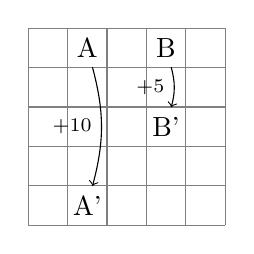
\begin{tikzpicture}
      \draw[step=0.5cm, color=gray] (0,0) grid (2.5,2.5);
      \node (A) at (0.75,2.25) {A};
      \node (A') at (0.75,0.25) {A'};
      \node (B) at (1.75,2.25) {B};
      \node (B') at (1.75,1.25) {B'};
      \draw [->][bend left=15] (A) edge node[left] {\scriptsize{+10}} (A');
      \draw [->][bend left=15] (B) edge node[left] {\scriptsize{+5}} (B');
    \end{tikzpicture}
    \caption{The simple gridworld Markov decision process.}
  \end{figure}
  The \emph{gridworld} MDP consist of 25 states $\cl{S} = [5]^2$ and 4 actions
  $\cl{A} = \{U, D, L, R\}$ for \emph{up}, \emph{down}, \emph{left} and 
  \emph{right}. The transition $P$ and reward $R$ kernels are deterministic:
  the agent moves 1 square up, down, left or right according to the chosen
  action and receives a reward of 0, except:
  \begin{itemize}
    \item Any move that would move the
      agent out of the grid results in no movement and a reward of -1.
    \item Any action in the state $A = (2,1)$ results in $A' = (2,5)$ as
      the next state and a reward of 10.
    \item Any action in the state $B = (4,1)$ results in $B' = (4,3)$ as
      the next state and a reward of 5.
  \end{itemize}
  Finite spaces are trivially standard Borel with the discrete topology,
  which also makes every map $(s, a) \mapsto \cl{X}$ into some
  topological space continuous. In particular $P$ is continuous and
  $r$ is (upper semi)continuous.
  The set of admissible actions $A(s)$ is equal to the
  full action space $\cl{A}$ for all $s \in \cl{S}$, which is trivially
  compact.
  The rewards are bounded by $R_{\max} = 10$.
  Setting $\gamma = 0.9$ makes (D) hold, and puts
  $V_{\max} = 10/(1-0.9) = 100$.
  Thus we can apply \cref{cor:Viteration} and for $\wt{V}_0 = 0$ get that
  \[ \abs{\wt{V}_K - V^*} \leq \gamma^K \abs{V^*}
  \leq \gamma^K V_{\max} = 100 \cdot 0.9^{-K} \]
  
  By \cref{prop:propTpiV} for any stationary policy $\tau \in S\Pi$ we have
  that $T_\tau$ is also $\gamma$-contractive and we
  easily get the same bound on the policy evaluation
  \[ \abs{T_\tau^k V_0 - V_\tau} \leq \gamma^K V_{\max} \]
  Measures over finite spaces can be represented as real vectors,
  and kernels as matrices.
  For example the transition kernel
  $P: \cl{P}(\cl{S} \times \cl{A}) \to \cl{P}(\cl{S})$
  is a $\abs{\cl{S}} \times (\abs{\cl{S}} \cdot \abs{\cl{A}})$-matrix.
  Calculating $TV$ and $T_\pi V$ is then a matter of matrix multiplication
  and taking maxima over vectors.

  Define the stationary policy $\tau_r(\cdot \mid \cdot) = \frac{1}{4}$ which
  chooses actions uniformly at random at every state.

  \begin{figure}[h]
    \centering
    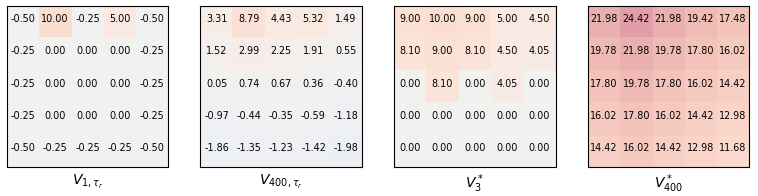
\includegraphics[scale=0.7]{figs/gridworld1.png}
    \caption{Value functions of the gridworld environment.}
  \end{figure}

  \label{ex:gridworld}
\end{example}

\subsection{Q-functions}
Throughout this section we assume \cref{sett:BS0}, (D) and furthermore that
$A(s)$ is finite for every $s \in \cl{S}$.

A \defemph{Q-function} is any function that assigns a (extended) real number
to every state-action pair, that is any function $Q : \cl{S} \times \cl{A}
\to \Rext$. Q-function are also called \emph{action-value} functions,
to distinguish them from the \emph{value} functions we have discussed in the
previous sections.
Because of the similar role Q-functions play compared to value function,
many concepts such as $T$-operators and the finite, infinite horizon
policy evaluations and greedy policies, can be defined analogously.

\begin{defn}[Policy evaluation for Q-functions]
  Let $\pi \in R\Pi$.
  Define
  \[ Q_{k, \pi}(s, a) = r(s, a) + \gamma \E_{P(\cdot \mid s, a)} V_{k, \pi}
  ,\qquad Q_\pi(s, a) = r(s, a) + \gamma \E_{P(\cdot \mid s, a)} V_\pi \]
  \[ Q^*_k = \sup_{\pi \in R\Pi} Q_{k, \pi}
  , \qquad Q^* = \sup_{\pi \in R\Pi} Q_\pi \]
  Define $Q_0 = r$ then we make the convention that
  $Q^*_0 = Q_{0,\pi} = Q_0 = r$.
  \label{defn:polEvalQ}
\end{defn}
\begin{defn}[Operators for Q-functions]
  For any stationary policy $\tau \in S\Pi$
  and measurable $Q:\Cal{S} \times \Cal{A} \to \ol{\ul{\R}}$ with
  $Q \geq 0, Q \leq 0$ or $\abs{Q} < \infty$ we define
  \[ P_\tau Q(s, a) = \int Q(s', a') \difd \tau P(s', a' \mid s, a) \]
  \[ T_\tau Q = r + \gamma P_\tau Q \]
  \[ T Q(s, a) = r(s, a) + \gamma
  \int \max_{a' \in \Cal{A}} Q(s', a') \difd P(s' \mid s, a) \]
  where $T_a = T_{\delta_a}$.
  \label{defn:opQ}
\end{defn}
\begin{rem}
  The $P_\tau$ operator is defined for simplications in proofs, especially
  in the analysis of \mcite{F20} in the later sections.
\end{rem}
\begin{defn}[Greedy policies for Q-functions]
  Let $\tau : \Cal{S} \leadsto \Cal{A}$ be a stationary policy. Define
  $G_Q(s) = \argmax_{a \in A(s)} Q(s, a)$.
  If there exist a measurable set $G_Q^\tau(s) \subseteq G_Q(s)$
  for every $s \in \Cal{S}$ such that
  \[ \tau \left( G_Q^\tau(s) \Mid s \right) = 1 \]
  then $\tau$ is said to be \defemph{greedy} with respect to $Q$ and is
  denoted $\tau_Q$.
  \label{defn:greedyQ}
\end{defn}

The idea of Q-functions (and the letter Q) originates to
\mcite{W89}. Upon the definition he notes
\begin{displayquote}
  ``This is much simpler to calculate than [$V_\pi$]
  for to calculate [$Q_\pi$] it is only necessary to look one
  step ahead [\ldots]''
\end{displayquote}
A clear advantage of working with Q-function
$Q:\Cal{S}\times\Cal{A} \to \Rext$ rather than a value function
$V:\Cal{S}\to \Rext$,
is that finding the optimal action in state $s$
requires only a maximization over the Q-function itself:
$a = \argmax_{a \in A(s)} Q(s,a)$.
This should be compared to finding a best action according to a value
function $V$:
$a = \argmax_{a \in A(s)} r(s,a) + \gamma \E_{P(\cdot \mid s,a)} V$.
Besides being less simple,
this requires taking an expectation with respect to 
both the reward and transition kernel.
Later we will study settings where we are not allowed to know
the process kernels when attempting to find the optimal strategy.
In these situations the advantage of Q-functions is clear.
For now however the transition kernel will remain known and we
will in this section see how the results of state-value functions
translate to Q-functions.

\begin{prop}[Relations between Q- and value functions]
  Let $\pi = (\tau_1, \tau_2, \dots) \in M\Pi$ be a Markov policy
  and $\tau \in S\Pi$ stationary. Then
  \leavevmode
  \begin{enumerate}
    \item Policy evaluations are related by
      $\E_{\tau(\cdot \mid s)} Q_{k, \pi} = V_{k+1, (\tau, \pi)}(s)$.
    \item $T_\tau$-operators are related by $T_\tau Q_{k, \pi}(s, a)
      = r + \gamma \E_{P(\cdot \mid s, a)} T_\tau V_{k, \pi}$.
    \item Greedy policies for policy evaluations are the same,
      that is
      \[ \tau(Q_{k, \pi}) = \tau(V_{k, \pi}), \; \mathrm{and} \;
      \tau(Q_\pi) = \tau(V_\pi) \]
    \item Optimal policies are related by
      $\max_{a \in A(s)} Q^*(s, a) = V^*(s)$ and
      \[ Q^*_k(s, a) = r(s, a) + \gamma \E_{P(\cdot \mid s, a)} V^*_k,
      \quad Q^*(s, a) = r(s, a) + \gamma \E_{P(\cdot \mid s, a)} V^* \]
    \end{enumerate}
  \label{prop:relQV}
\end{prop}

\begin{prop}[Properties of Q-functions]
  Let $\pi = (\tau_1, \tau_2, \dots) \in M\Pi$ be a Markov policy
  and $\tau \in S\Pi$ stationary. Then
  \leavevmode
  \begin{enumerate}
    \item $Q_{k, \pi} = T_{\tau_1} \dots T_{\tau_k} Q_0$ and
      $Q^*_k = T_{\tau_{k-1}^*} \dots T_{\tau_0^*} Q^*_0
      = T^k Q^*_0$.
    \item $Q_\pi = \lim_{k \to \infty} Q_{k, \pi}$ and
      $Q^* = \lim_{k\to\infty} Q_k^*$. 
    \item $T,\; T_\tau$ are $\gamma$-contractive on
      $\Cal{L}_\infty(\Cal{S}\times\Cal{A})$
      and $Q^*,\; Q_\tau$ are their unique fixed points.
    \item $Q^* = Q_{\tau^*}$ and
      $Q_{k, \pi},\; Q_\pi,\; Q^*_k,\; Q^*$ are all upper semicontinuous
      and bounded by $V_{\max}$.
  \end{enumerate}
  \label{prop:propQ}
\end{prop}

\begin{proof}[Proof of \cref{prop:relQV} and \cref{prop:propQ}]
%todo fix this proof
  Measurability of $Q_{k, \pi}$ and $Q_\pi$
  follow from measurability of $V_{k, \pi}$, $V_{\pi}$
  and \cref{prop:intKerMeas}.
  Upper semicontinuity of $Q_{k, \pi}$ and $Q_\pi$ follows
  from \cref{prop:intSemiC} because $V_{k, \pi}$ and $V_\pi$ are
  upper semicontinuous (see \cref{cor:Viteration}).

  For \cref{prop:relQV}.1 we have \begin{align*}
    \E_{\tau(\cdot \mid s)} Q_{k, \pi}
    &= \int r(s,a) + \gamma \E_{P(\cdot \mid s, a)} V_{k, \pi}
    \difd \tau(a \mid s)
    \\ &= \int r(s,a) + \gamma \sum_{i=1}^{k} \gamma^{i-1} r(s_i, a_i)
    \difd P \tau_k \dots P\tau_1 P\tau(a, s_1, a_1, \dots, s_k \mid s)
  \\ &= V_{k+1, (\tau, \pi)} \end{align*}
  
  For \cref{prop:relQV}.2 we sketch the idea by
  \begin{align*}
    T_\tau Q_{k, \pi} = r + \gamma \int r + \gamma V_{k, \pi}
    \difd P \difd \tau P
    = r + \gamma \int r + \gamma V_{k, \pi} \difd P \tau \difd P
    = r + \gamma \int T_\tau V_{k, \pi} \difd P
  \end{align*}
  
  For $Q_{k,\pi} = T_{\tau_1} \dots T_{\tau_k} Q_0$ use \cref{prop:relQV}.2
  iteratively starting with
  $\tau = \tau_1, \pi = (\tau_2, \tau_3, \dots)$.
  
  The $\tau(Q_{k, \pi}) = \tau(V_{k, \pi})$ part of \cref{prop:relQV}.3
  is by definition of the two concepts of
  greedy functions.

  That $Q_\pi = \lim_{k \to \infty} Q_{k, \pi}$
  follows from dominated convergence and
  \cref{prop:VpiMeas}.3.

  For \cref{prop:relQV}.4 $Q_k^* = \sup_{\pi \in R\Pi} (r + \gamma \E V_{k,\pi})
  \leq r + \gamma \E V_k^* = r + \gamma \E V_{\pi_k^*}
  \leq Q_k^*$. The same argument works for the second part.

  Let $s \in \Cal{S}$ then $\sup_{a \in A(s)} Q^*(s, a) = 
  \sup_{a \in A(s)} (r(s, a) + \gamma \E_{P(\cdot \mid s, a)} V^*)
  = T V^*(s) = V^*(s)$.
  
  By the definition of $Q_{\tau^*}$ we have
  $Q^* = r + \gamma \E V^* = r + \gamma \E V_{\pi^*} = Q_{\tau^*}$.

  $T_\tau Q_\tau = T_\tau (r + \gamma \E \lim_{k\to\infty} T_\tau^k V_0)
  = \lim_{k\to\infty} T_\tau (r + \gamma \E T_\tau^k V_0)
  = \lim_{k\to\infty} (r + \gamma \E T_\tau^{k+1} V_0)
  = r + \gamma \E \lim_{k\to\infty} T^{k+1}_\tau V_0
  = r + \gamma \E V_\tau = Q_\tau$.

    We $T_{\tau_Q} Q = T Q$ for any measurable $Q$ because
  \[ T_{\tau_Q}(s, a) = r(s, a) + \gamma \int \max_{a' \in A(s')} Q(s', a')
  \difd P(s' \mid s, a) = TQ(s, a) \]
  Therefore by \cref{prop:propQ}.1
  \[ T_{\tau_{k-1}^*} Q_{k-1, (\tau_{k-2}^*, \dots, \tau_0^*)}
  = T Q_{k-1}^* \]
  since by \cref{prop:relQV}.3 $\tau_{k-1}^*$ is greedy for $Q_{k-1}^*$.
  Now use induction to get $Q^*_{k-1} = T^k Q_0^*$.

  Because $V^* = V_{\tau^*}$ we have
  \[ TQ^* = T_{\tau^*} = r + \gamma \E T_{\tau^*} V_{\tau^*}
  = r + \gamma \E V^* = Q^* \]

  The contrativeness of $T$ and $T_\pi$ follows from the same argument as for
  value functions.
  Banach fixed point theorem now concludes \cref{prop:propQ}.3.

  Since now $Q^*$ and $Q_{\tau^*}$ are fixed points for $T$ they must be
  equal, concluding the last point, namely \cref{prop:propQ}.4.
\end{proof}

\begin{cor}
  For any $Q \in \Cal{L}_\infty(\Cal{S} \times \Cal{A})$
  $T^k Q$ converges to $Q^*$ with rate $\gamma^k$.
  That is
  \[ \abs{T^k Q - Q^*} \leq \gamma^k \abs{Q - Q^*} \]
  \label{cor:QrateSimple}
\end{cor}
\begin{proof}
  By \cref{prop:propQ}.3.
\end{proof}

\subsection{Q-iteration}

Similar to the value iteration algorithm (\cref{alg:valueIteration}) we can
define the corresponding for Q-iteration.

\begin{figure}[H]
\begin{algorithm}[H] %\label{algocf:fq} % this labels line, could not fix
\caption{Simple theoretical Q-iteration}
\KwIn{MDP $(\Cal{S}, \Cal{A}, P, R, \gamma)$, number of iterations $K$}
$r \leftarrow \int x \difd R(x \mid \cdot)$

$\wt{Q}_0 \leftarrow r$

\For{$k = 0,1,2,\dots,K-1$}{
  $ \wt{Q}_{k+1} \leftarrow r
  + \gamma \int \sup_{a' \in \Cal{A}} \wt{Q}_k(s', a') \difd P(s' \mid \cdot)$
}
\KwOut{An estimator $\widetilde{Q}_K$ of $Q^*$}
\label{alg:theoSimpleQ}
\end{algorithm}
\end{figure}

\begin{prop}(D)

  The output $\wt{Q}_K$ of \cref{alg:theoSimpleQ} converges to the optimal
  Q-function $Q^*$ with rate $\gamma^K$ concretely
  $\norm{\wt{Q}_K - Q^*}_\infty \leq \gamma^K \norm{Q^*}_\infty$.
  \label{prop:theoSimpleQConv}
\end{prop}
\begin{proof}
  This is by \cref{cor:QrateSimple}.
\end{proof}

\subsubsection{Finite Q-iteration}
We have shown how if one knows the dynamics
of a stationary decision process satisfying rather broad criteria, 
such as continuity and compactness,
the optimal policy and state-value function can be found
simply by iteration over the $T$-operator and picking a greedy strategy
(see \cref{prop:theoSimpleQConv}).
Of course this is practical computationally, only if
the resulting $Q$ functions can be represented and computed in finite
space and time.
An obvious situation in which such a representation and computation is possible,
is the finite case.
Say $\abs{\Cal{S}} = k$ and $\abs{\Cal{A}} = \ell$.
In this case the transition operator $P$ can be represented as a
matrix of \emph{transition probabilities}
\[ P \defeq \begin{pmatrix}
    P(s_1 \mid s_1, a_1) & \dots & P(s_k \mid s_1, a_1)
    \\ \vdots & \vdots & \vdots
    \\ P(s_1 \mid s_k, a_\ell) & \dots & P(s_k \mid s_k, a_\ell)
\end{pmatrix} \]
then the algorithm becomes

\begin{algorithm}[H] %\label{algocf:fq} % this labels line, could not fix
\caption{Simple finite Q-iteration}
\KwIn{MPD $(\Cal{S}, \Cal{A}, P, R, \gamma)$, number of iterations $K$}
Set $ r \leftarrow \left(\int r \difd R(r \mid s_1, a_1),
\dots, \int r \difd R(r \mid s_k, a_\ell) \right)^T $

and $ \wt{Q}_0 \leftarrow r$.

\For{$k = 0,1,2,\dots,K-1$}{
  Set $m(\wt{Q}_k) \leftarrow (\max_{a \in \Cal{A}} Q(s_1, a), \dots,
  \max_{a \in \Cal{A}}Q(s_k, a))^T$

  Update action-value function:
  \[ \wt{Q}_{k+1} \leftarrow
    r + \gamma P m(\wt{Q}_k)
  \]
}
\KwOut{An estimator $\widetilde{Q}_K$ of $Q^*$}
\label{alg:finiteSimpleQ}
\end{algorithm}

\begin{prop}
  The output $\wt{Q}_K$ from \cref{alg:finiteSimpleQ} is
  $K$-optimal and
  $\norm{\wt{Q}_K - Q^*}_\infty \leq \gamma^K \norm{Q^*}_\infty$.
\end{prop}
\begin{proof}
  See \cref{cor:QrateSimple}.
\end{proof}

\section{Approximation}
In this section we will look at what happens if we
instead use approximations of the Q-functions and $T$ operator.
This means that we are in a setting where we can somehow
calculate $r$ and $TQ$ for any $(s,a) \in \cl{S} \times \cl{A}$,
but it is hard or infeasible to represent them (or at least one of them)
directly.
This setting is not very well-studied in the case of a
continuous state space (at least in the sources known to this writer).
This is perhaps because it is considered solved
by the results of theoretical Q-learning presented in the previous section.
However as we have argued, this only have practical relevance 
when it is feasible to represent $TQ$.
Therefore we find it relevant to consider this setting in more detail.
What \emph{is} very well-studied is a further generalized setting
where $T$ and $r$ are assumed to be unknown,
that is, one has only access to their distributions via sampling from them.
We will deal with this setting in the next section.
In following we present some rather simple bounding techniques
which is inspired by arguments found in e.g. \ncite{F20},
together with some standard results from approximation theory
on artificial neural networks and Bernstein polynomials.
Throughout this section we assume (D)
i.e. that we are discounting with some $\gamma \in [0,1)$.

Let us consider any norm $\norm{\cdot}$ on
$(\cl{F}, \norm{\cdot})$ where $\cl{F} \subseteq \cl{Q}$ is
a subset of the space of bounded
Q-functions $\cl{Q} = \cl{L}_\infty(\cl{S}\times\cl{A})$.
Let $\wt{Q}_0$ be any Q-function which is bounded in $\norm{\cdot}$.
Suppose we approximate $T\wt{Q}_0$ by a Q-function $\wt{Q}_1$
to $\ve_1 > 0$ precision and then approximate $T\wt{Q}_1$ by $\wt{Q}_2$
and so on. This way we get a sequence of Q-functions satisfying
\[ \norm{T\wt{Q}_{k-1} - \wt{Q}_k} \leq \ve_k, \forall k \in \N \]

First observe that
\begin{align*}
  \norm{T^k \wt{Q}_0 - \wt{Q}_k}
  &\leq \norm{T^k \wt{Q}_0 - T \wt{Q}_{k-1}} + \norm{T\wt{Q}_{k-1} - \wt{Q}_k}
  \\ &\leq \gamma \norm{T^{k-1} \wt{Q}_0 - \wt{Q}_{k-1}}
  + \norm{T\wt{Q}_{k-1} - \wt{Q}_k}
\end{align*}

Using this iteratively we get
\[ \norm{T^k \wt{Q}_0 - \wt{Q}_k} \leq \sum_{i=1}^k \gamma^{k-i} \ve_i
\defeq \ve_{\mathrm{approx}}(k) \]

Then we can bound
\begin{align*}
  \norm{Q^* - \wt{Q}_k}
  &\leq \norm{Q^* - T^k \wt{Q}_0} + \norm{T^k \wt{Q}_0 - \wt{Q}_k}
  \\ &\leq \gamma^k \norm{Q^* - \wt{Q}_0}
  + \ve_{\mathrm{approx}}(k)
\end{align*}

These terms are called respectively the \emph{algorithmic} error
and the \emph{approximation} error.

The algorithmic error converges exponentially, so one is often happy with this
part not spending time trying to bound this tighter.
The approximation error depends on our step-wise approximations. For example
if $\ve_i(k) = \ve$ for some $\ve > 0$ we easily get the bound
\begin{equation}
  \ve_{\mathrm{approx}}(k) = \ve \frac{1-\gamma^k}{1-\gamma} \leq \frac{\ve}{1-\gamma}
  \label{eq:approxEpsBound}
\end{equation}
If $\ve_i \leq c\gamma^i$ we get $\ve_{\mathrm{approx}}(k) \leq ck \gamma^k \to 0$ as
$k \to \infty$.
Generally if one can show that $\ve_i \to 0$ we have
\begin{prop} $ \sum_{i-1}^k \gamma^{k-i} \ve_i \to 0 $
  whenever $\ve_k \to 0$ as $k \to \infty$.
\end{prop}
\begin{proof}
  Let $\ve > 0$. Find $N$ such that $\ve_n \leq \ve (1-\gamma)/2$ 
  for all $n>N$ and find $M>N$ such that
  $\gamma^M \leq
  \ve \gamma^N \left( \sum_{i=1}^N \gamma^{N-i} \ve_i \right)^{-1}$.
  Then for all $m>M$
  \begin{align*}
    \sum_{i=1}^m \gamma^{m-i} \ve_i
    &\leq \gamma^{m-N} \sum_{i=1}^N \gamma^{N-i} \ve_i
    + \sum_{i=N+1}^m \gamma^{m-i} \ve (1-\gamma)/2
    \leq \ve/2 + \ve/2 \leq \ve
  \end{align*}
\end{proof}

\subsection{Using artifical neural networks}

\begin{sett}
  An MDP $(\cl{S}, \cl{A}, P, R, \gamma)$ with
  $\cl{S} = [0,1]^w$ and $\cl{A}$ finite.
  Assume that $r$ is continuous and
  $P$ is setwise-continuous.
  \label{sett:annApprox}
\end{sett}

\begin{defn}\label{def_ANN}
  An \textbf{ANN} (Artificial Neural Network) with structure
  $(d_i)_{i=0}^{L+1} \subseteq \N$,
  activation functions $\sigma_i = (\sigma_{ij})_{j=1}^{d_i}$, where
  $\sigma_{ij} : \R \to \R$ are real-valued functions on $\R$,
  and weights $W_i \in M^{d_i \times d_{i-1}}, \; v_i \in \R^{d_i}, \;
  i \in [L+1]$
  is the function $F:\R^{d_0} \to \R^{d_{L+1}}$ 
  \[ F = w_{L+1} \circ \sigma_L \circ w_L
  \circ \sigma_{L-1} \circ \dots \circ w_1 \]
  where $w_i$ is the affine function $x \mapsto W_i x + v_i$ for all $i$.
\end{defn}

To clarify we have $\sigma_i(x_1, \dots, x_{d_i})
= (\sigma_{i1}(x_1), \dots, \sigma_{id_{i}}(x_{d_{i}}))$.
$L \in \N_0$ is interpreted as the number of \emph{hidden layers} and
$d_i$ is the number of neurons or nodes in layer $i$.

We denote the class of these networks (or functions)
\[ \cl{DN} \left(\sigma_{ij}, ( d_i )_{i=0}^{L+1} \right) \]

An ANN is called \emph{deep} if there are two or more hidden layers.

%Todo note that ANNs imbed nicely in each other

\begin{thm}[Universal Approximation Theorem for ANNs]
  Let $\sigma: \R \to \R$ be non-constant, bounded and continuous
  activation function.
  Let $\ve > 0$ and $f \in C([0,1]^w)$.
  Then there exists an $N \in \N$ and a network
  $F \in \cl{DN}(\sigma, (w, N, 1))$
  with one hidden layer
  and activation function $\sigma$ such that
  \[ \norm{F - f}_\infty < \ve \]
  In other words $\bigcup_{N \in \N} \cl{DN}(\sigma, (w, N, 1))$ is
  dense in $C([0,1]^w)$.
  \label{thm:uniApprox}
\end{thm}
\begin{proof}[Discussion of proofs]
  The original proof in \mcite{C89} is very short and elegant,
  but non-constructive,
  using the Riesz Representation and Hahn-Banach theorems to
  obtain a contractiction to the statement that
  $\bigcup_{N \in \N} \cl{DN}(\sigma, (w,N,1))$
  is dense in $C([0,1]^w)$.
  Furthermore it considered only \emph{sigmoidal} activations
  functions, meaning that $\sigma$ should satisfy
  \[ \sigma(x) \to \begin{cases} 0 & x \to -\infty
  \\ 1 & x \to \infty \end{cases} \]
  
  This was extended in \mcite{CCR90} to the statement as presented above
  and their proof is constructive. 
\end{proof}

\begin{prop}
  Consider \cref{sett:annApprox} let
  and $\sigma : \R \to \R$ be a non-constant, bounded, continuous
  activation function. Let $\varepsilon > 0$.
  Then for every $k \in \N$ there exists a $N\in \N$ and a sequence of
  Q-networks $(\wt{Q}_i)_{i=1}^k \subseteq \cl{DN}(\sigma,
  \{w \abs{\cl{A}}, N, 1\})$ such that
  \[ \norm{T\wt{Q}_{i-1} - \wt{Q}_i}_\infty < \ve \]
  for all $i \in [k]$.
  In particular
  \[ \norm{Q^* - \wt{Q}_k}_\infty < \varepsilon/(1 - \gamma) \]
\end{prop}

This gives us the first method of how to approximate
$Q^*$ arbitrarily closely on continuous state spaces, in the case
where it is infeasible to represent $TQ$ directly.
To use this method in practice one would need to go through the
construction in \ncite{CCR90}. We will not go further into this,
and instead focus on another approximation method using
\emph{Bernstein polynomials}.

\subsection{Using Bernstein polynomials}

In this case the need a slightly stronger form of continuity, namely
Lipschitz continuity, to establish the bounds.

\begin{sett}
  An MDP $(\cl{S}, \cl{A}, P, R, \gamma)$ with
  $\cl{S} = [0,1]^w$ and $\cl{A}$ finite.
  Assume that there exists a probability measure $\mu \in \cl{S}$, such that
  $P(\cdot \mid s, a)$ has density
  $p(\cdot \mid s, a) : \cl{S} \to \R$ with respect to
  $\mu$ for all $(s, a) \in \cl{S}\times\cl{A}$. 
  Furthermore assume that $r(\cdot, a), \; p(s \mid \cdot, a)$ are
  Lipschitz
  with constants $L_r,\; L_p$ respectively for all
  $(s, a) \in \cl{S} \times \cl{A}$.
  \label{sett:polyApprox}
\end{sett}

\begin{defn}[Bernstein polynomial]
  The multivariate Bernstein polynomial $B_{f, n}$ with exponents
  $n=(n_1, \dots, n_w) \in \N^w$ approximating the function $f:[0,1]^w \to \R$
  is defined by
  \begin{equation*}
    B_{f, n}(x_1, \dots, x_w) =
    \sum_{j = 1}^w \sum_{k_j = 0}^{n_j}
    f\left( \frac{k_1}{n_1}, \dots, \frac{k_w}{n_w} \right)
    \prod_{\ell = 1}^w \left(
    \binom{n_\ell}{k_\ell} x_\ell^{k_\ell}(1-x_\ell)^{n_\ell - k_\ell} \right)
  \end{equation*}
  \label{defn:Bfn}
\end{defn}
Notice that this a polynomial of (multivariate) degree $n_1 + \dots + n_w$.

\begin{thm}
  Let $f : [0,1]^w \to \R$ be Lipschitz (see \cref{defn:Lipschitz})
  w.r.t. the standard euclidean 2-norm induced metrics on $[0,1]^w$ and $\R$
  with constant $L$. 
  Then for any $n = (n_1, \dots, n_w) \in \N^w$ there exists a polynomial
  $B_{f,n} : [0,1]^w \to \R$ of degree $\leq \norm{n}_1$ such that
  \begin{enumerate}
    \item $\norm{f - B_{f,n}}_2
      \leq \frac{L}{2} \sqrt{\sum_{j=1}^w \frac{1}{n_j}}$
    \item $\norm{B_{f,n}}_\infty \leq \norm{f}_\infty$
  \end{enumerate}
\end{thm}

\begin{lem}
  $TQ(\cdot, a)$ is Lipschitz in $\norm{\cdot}_2$ with constant
  $ L_T = (L_r + \gamma V_{\max} L_p) $
  for all $a \in \cl{A}$ and $Q : \cl{S} \times \cl{A} \to [-V_{\max},V_{\max}]$.
\end{lem}

Now we can bound

\begin{prop}
  \[ \ve_{\mathrm{approx}} \leq \frac{L_r + \gamma V_{\max} L_p}{2(1-\gamma)}
  \sqrt{\sum_{j=1}^w \frac{1}{n_j}} \]
\end{prop}

For example if we put $n_j = m$ for all $j$ we get

\begin{prop}
  \[ \norm{Q^* - \wt{Q}_k} \leq \norm{Q^* - \wt{Q}_0}
    + \frac{L_r + \gamma V_{\max} L_p}{2(1-\gamma)} \sqrt{w}
  m^{-1/2} \]
  In particular $\norm{Q^* - \wt{Q}_k}_\infty
  = \cl{O}(\gamma^{-k} + \frac{1}{\sqrt{m}})$
  when using $k$ iterations and approximating
  with multivariate polynomials of maximum degree $w \cdot m$.
\end{prop}

This gives a very concrete way of constructing an arbitrarily good
approximation to $Q^*$ using polynomials.
%todo example.



